\section{The 3-Dimensional Case - N-Units Away Surfaces}

One last thing I want to mention is that you can, with only minimal effort, extend almost all of the ideas covered in this paper to higher dimensional arenas. Where before we were taking a function $y = f(x)$ and moving one unit away along every normal line to that function, now take a surface $z = f(x,y)$ and move one unit away from it along every normal line.

Instead of $f_N(t) = \begin{bmatrix} t \\ f(t) \end{bmatrix} + N \dfrac{\langle -f'(t), 1 \rangle}{|\langle -f'(t), 1 \rangle|}$, now we have $f_N(u, v) = \begin{bmatrix} u \\ v \\ f(u, v) \end{bmatrix} + N \dfrac{\langle -\dfrac{df}{dx}, -\dfrac{df}{dy}, 1 \rangle}{|\langle -\dfrac{df}{dx}, -\dfrac{df}{dy}, 1 \rangle|}$.

Running this into the Pacific Tech Graphing Calculator, one gets a glimpse at the marvelous and humorous world of $N$-Units Away Surfaces! Here is the graph of the $N$-Units Away Surfaces for $f(x,y) = sinx + siny$:

\begin{figure}[H] 
  \label{surface-1} 
  \centering
  \begin{minipage}[b]{0.3\linewidth}
    \centering
    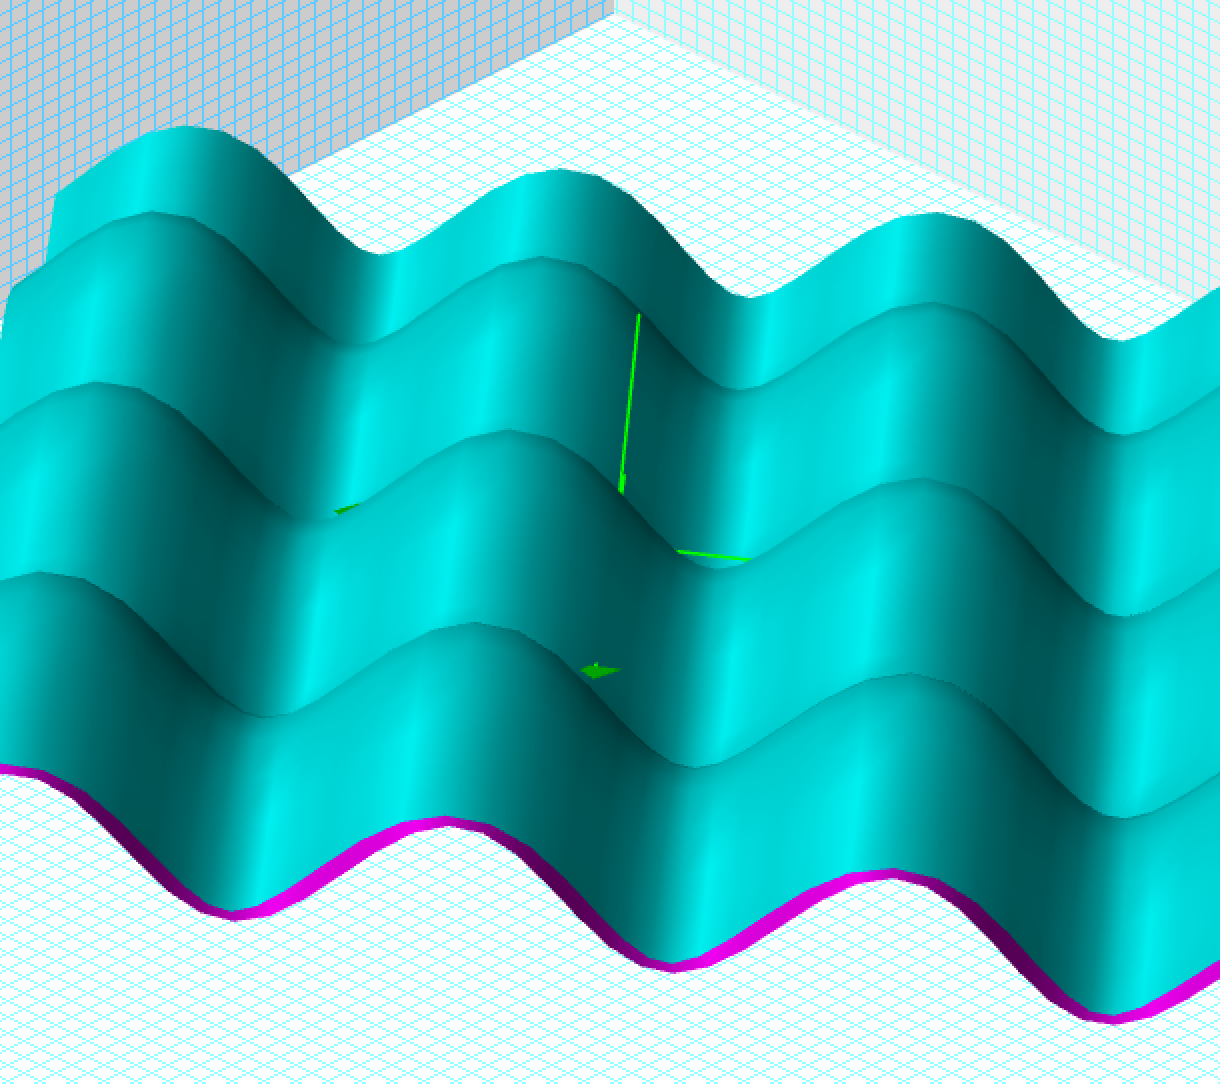
\includegraphics[width=.9\linewidth]{surfaces-img/Fig 39.png} 
    \caption{Caption} 
    \label{fig:fig39}
    \vspace{4ex}
  \end{minipage} % end 
  \begin{minipage}[b]{0.3\linewidth}
    \centering
    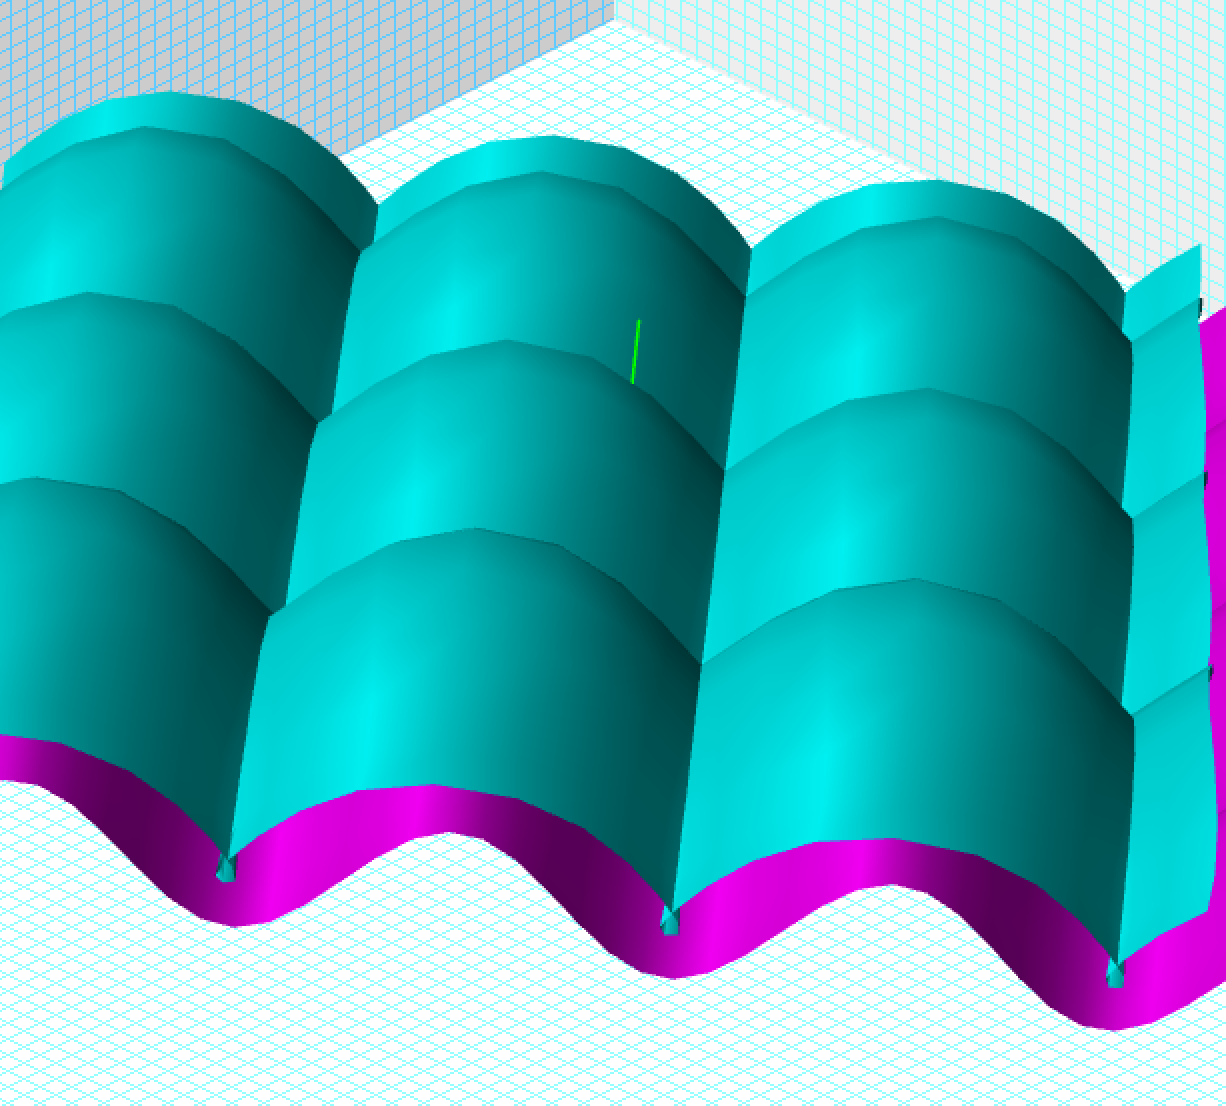
\includegraphics[width=.9\linewidth]{surfaces-img/Fig 40.png} 
    \caption{Caption} 
    \label{fig:fig40}
    \vspace{4ex}
  \end{minipage} % end
  \begin{minipage}[b]{0.3\linewidth}
    \centering
    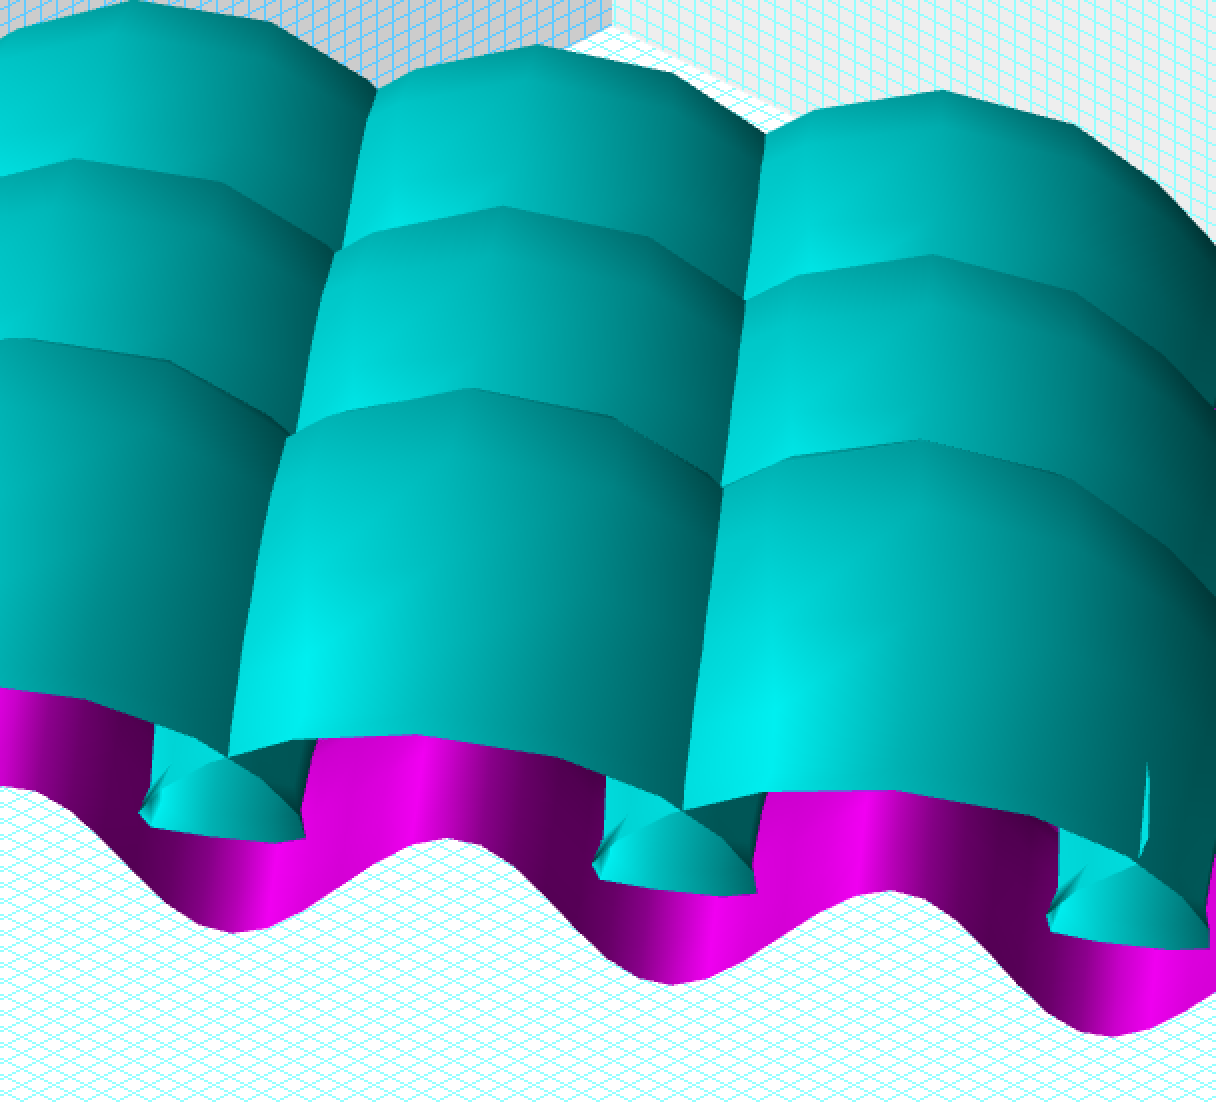
\includegraphics[width=.9\linewidth]{surfaces-img/Fig 41.png} 
    \caption{Caption} 
    \label{fig:fig41}
    \vspace{4ex}
  \end{minipage} % end
  \begin{minipage}[b]{0.3\linewidth}
    \centering
    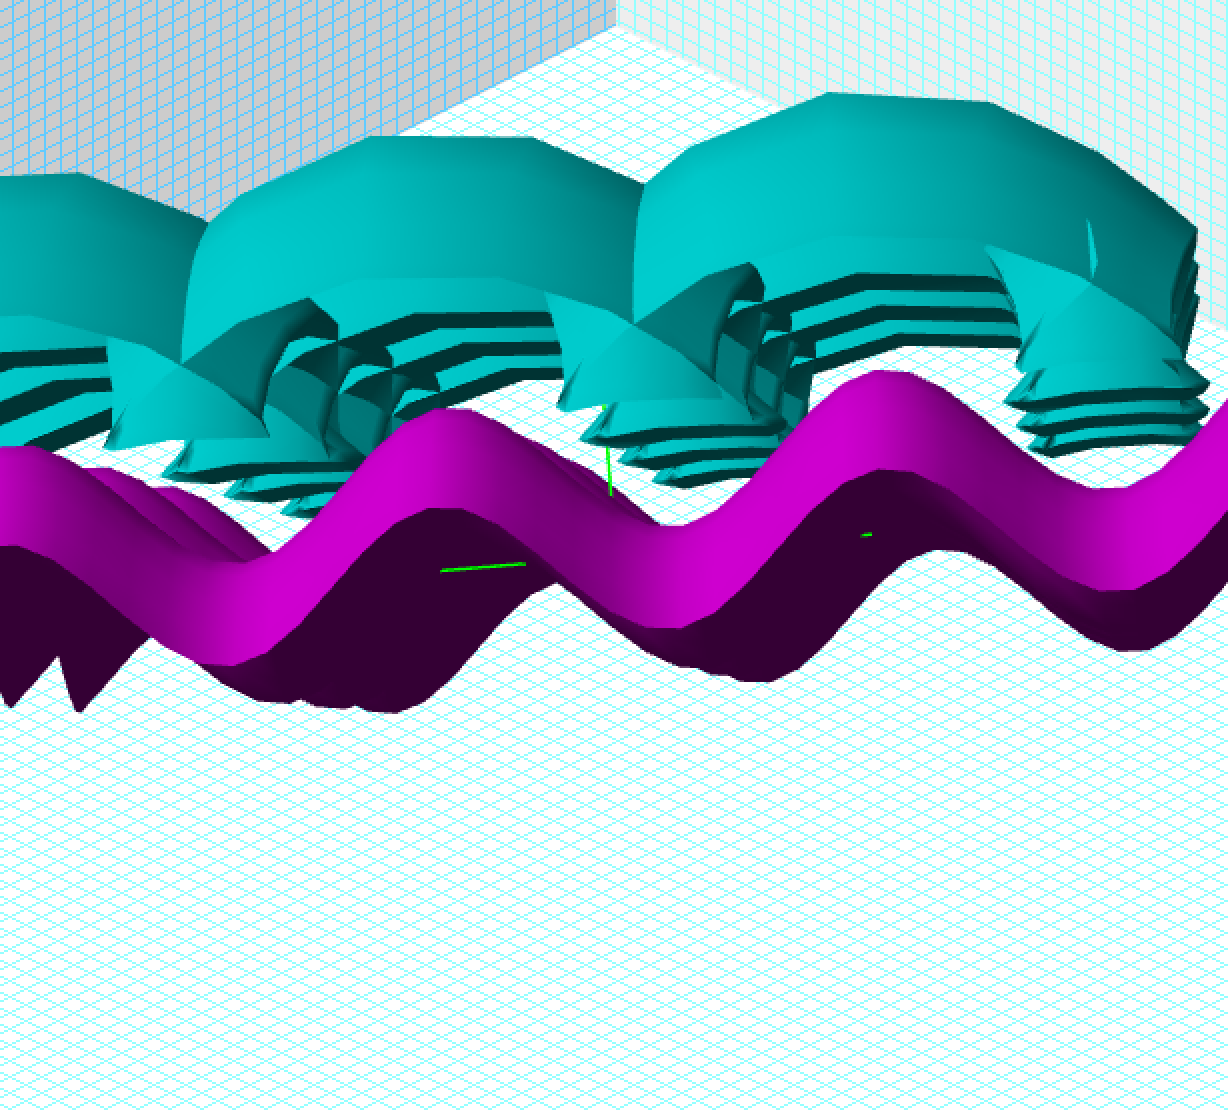
\includegraphics[width=.9\linewidth]{surfaces-img/Fig 42.png} 
    \caption{Caption} 
    \label{fig:fig42}
    \vspace{4ex}
  \end{minipage} % end
  \begin{minipage}[b]{0.3\linewidth}
    \centering
    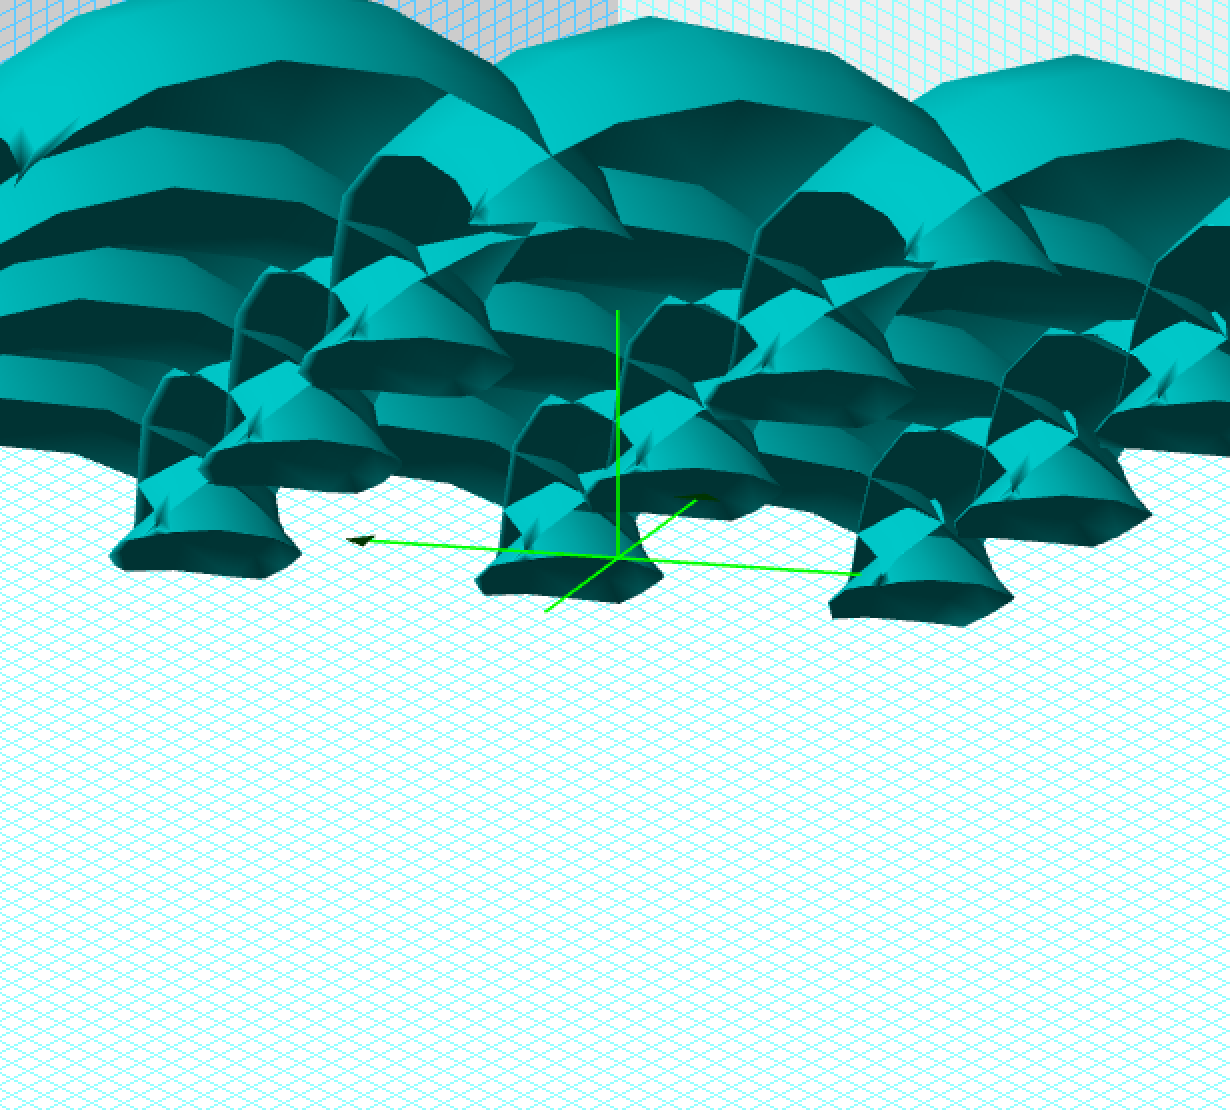
\includegraphics[width=.9\linewidth]{surfaces-img/Fig 43.png} 
    \caption{Caption} 
    \label{fig:fig43}
    \vspace{4ex}
  \end{minipage} % end
\end{figure}

While these are the N-Units Away Surfaces for $f(x,y) = atan(x) + sin(y)$:

\begin{figure}[H] 
  \label{surface-2} 
  \begin{minipage}[b]{0.5\linewidth}
    \centering
    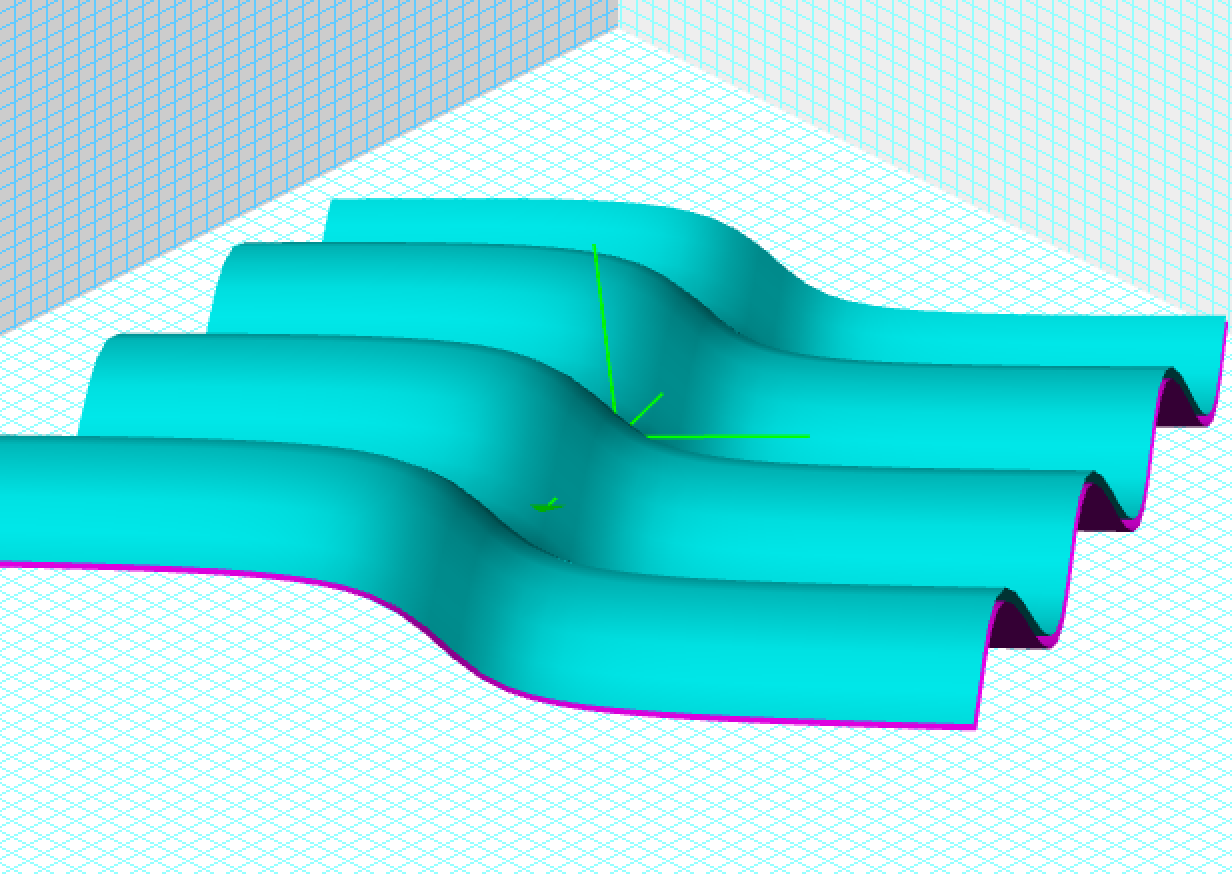
\includegraphics[width=.9\linewidth]{surfaces-img/Fig 44.png} 
    \caption{Caption} 
    \label{fig:fig44}
    \vspace{4ex}
  \end{minipage} % end 
  \begin{minipage}[b]{0.5\linewidth}
    \centering
    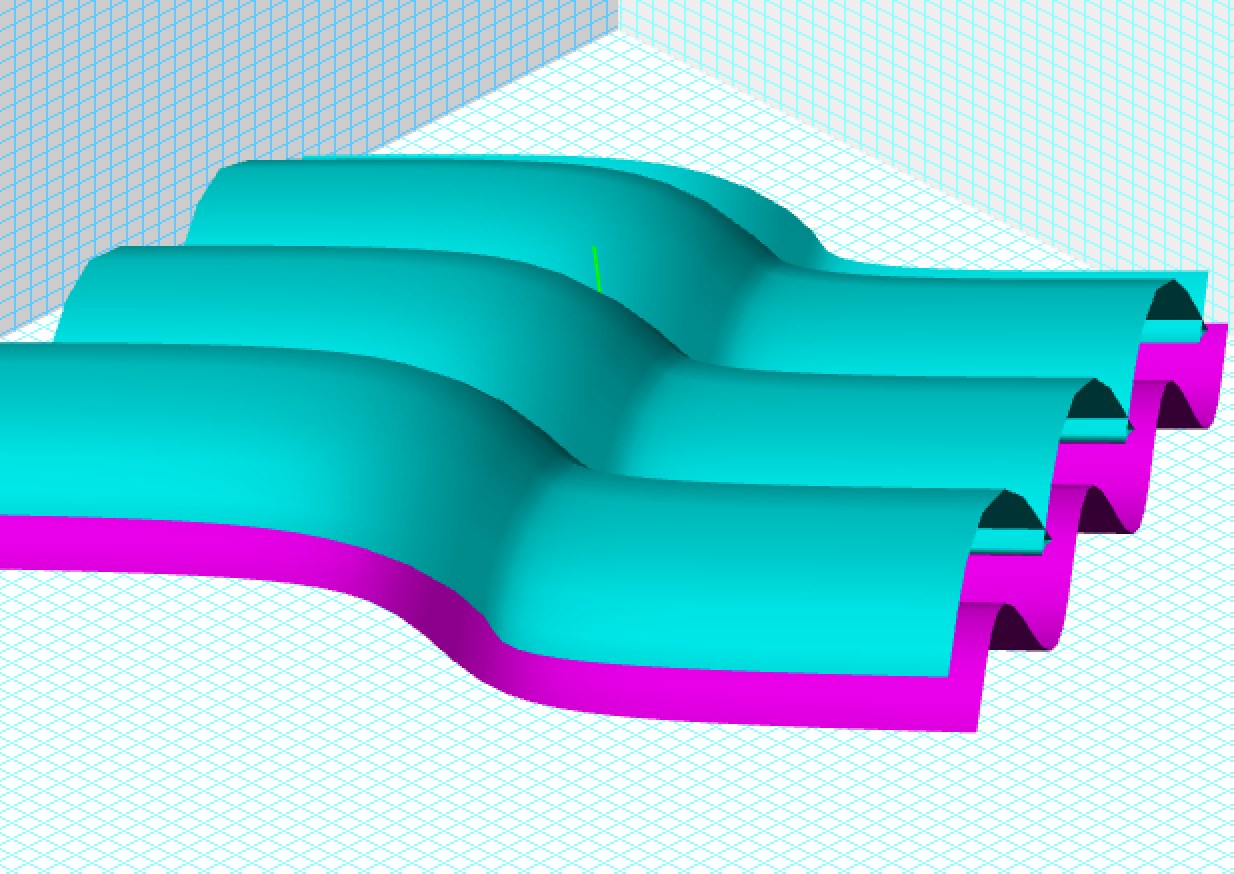
\includegraphics[width=.9\linewidth]{surfaces-img/Fig 45.png} 
    \caption{Caption} 
    \label{fig:fig45}
    \vspace{4ex}
  \end{minipage} % end
  \begin{minipage}[b]{0.5\linewidth}
    \centering
    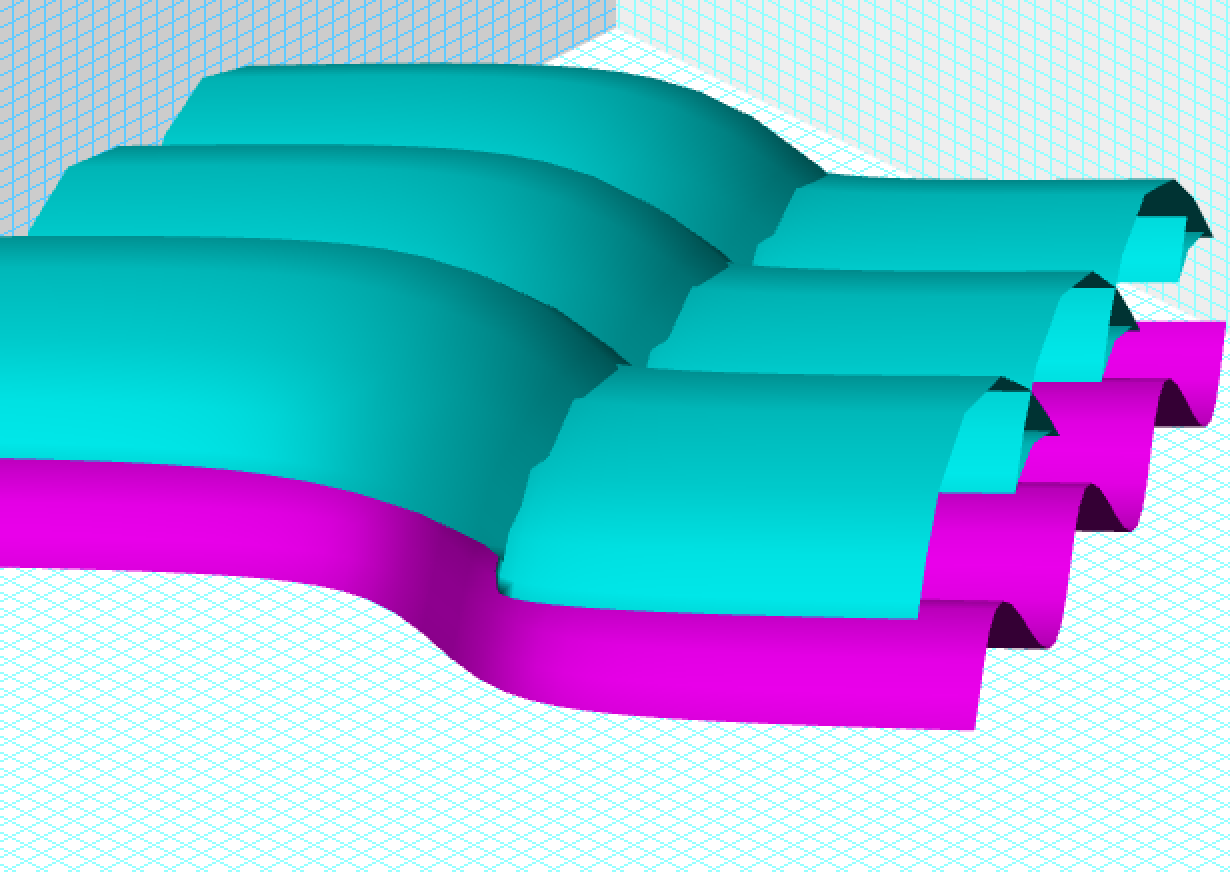
\includegraphics[width=.9\linewidth]{surfaces-img/Fig 46.png} 
    \caption{Caption} 
    \label{fig:fig46}
    \vspace{4ex}
  \end{minipage} % end
  \begin{minipage}[b]{0.5\linewidth}
    \centering
    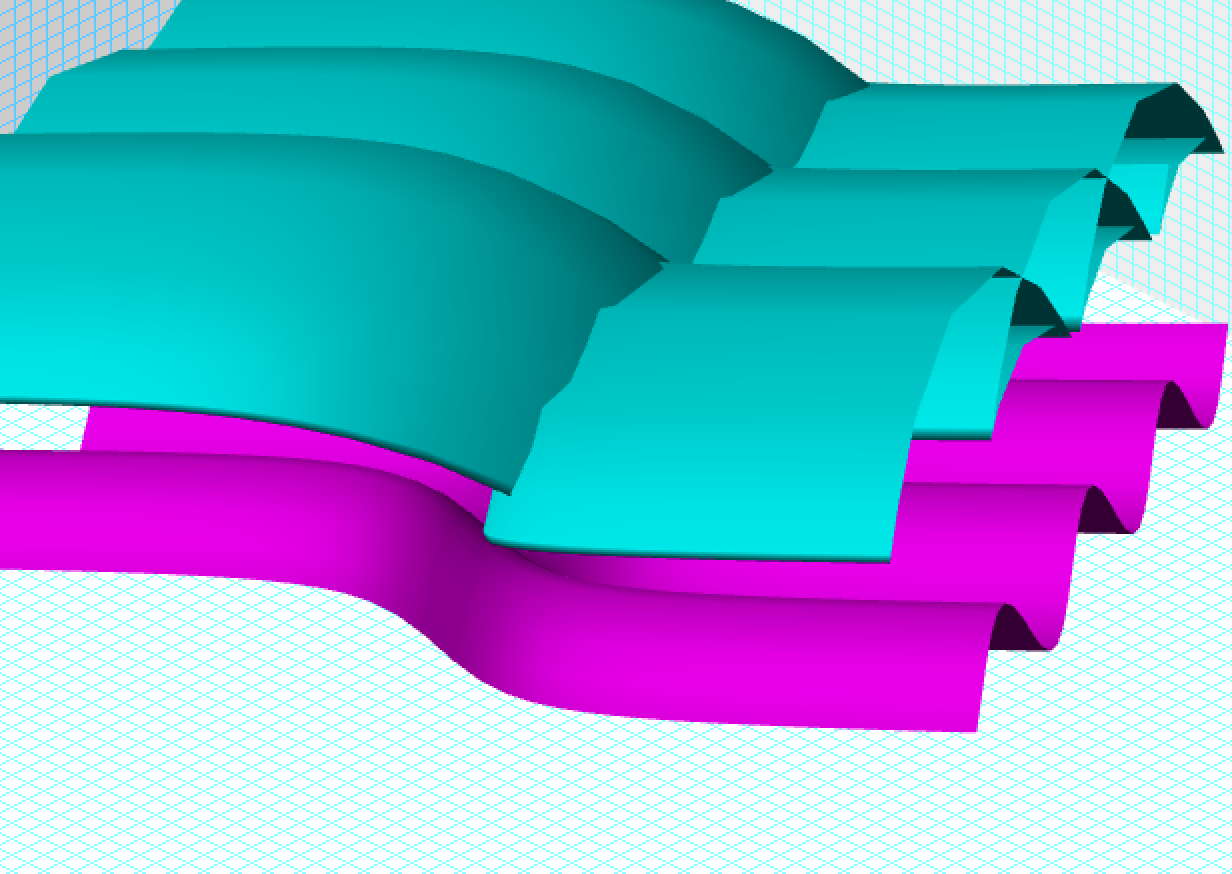
\includegraphics[width=.9\linewidth]{surfaces-img/Fig 47.png} 
    \caption{Caption} 
    \label{fig:fig47}
    \vspace{4ex}
  \end{minipage} % end
\end{figure}